\documentclass{article}

\usepackage{minitoc}
\usepackage{tabularx}
\usepackage{booktabs}
\usepackage{graphicx}
\usepackage{hyperref}
\usepackage{xcolor}
\usepackage{blkarray}
\usepackage{amsthm, amssymb, amsmath}
\usepackage{caption}
\usepackage{subcaption}
\usepackage{multirow}
\usepackage[ruled,vlined]{algorithm2e}

\usepackage{natbib}
\bibliographystyle{abbrvnat}

\theoremstyle{definition}
\newtheorem{definition}{Definition}[section]
\newtheorem{theorem}{Theorem}[section]
\newtheorem{lemma}[theorem]{Lemma}
\newtheorem{conjecture}[theorem]{Conjecture}

\usepackage[margin=2.5cm, includefoot, footskip=0pt]{geometry}
\pagestyle{plain}
\setlength{\parindent}{0em}
\setlength{\parskip}{1em}

\renewcommand{\baselinestretch}{1}

\newcommand{\nikoleta}[1]{\textcolor{teal}{{\bf NG:} #1}}

\newtheorem{proposition}{Proposition}

\title{\vspace{-2cm} Good reactive strategies in the iterated prisoner's dilemma}

\author{Nikoleta E. Glynatsi, Christian Hilbe, Martin Nowak}
\date{}

\begin{document}

\maketitle

\vspace{-.5cm}

We consider the infinitely repeated prisoner's dilemma with two players, denoted
as \(p\) and \(q\). At each turn, players \(p\) and \(q\) can choose between two
actions; cooperate (\(C\)) or defect (\(D\)). A player who cooperates pays a
cost \(c > 0\) to provide a benefit \(b > c\) for the co-player. A cooperator
either gets \(b - c\) (if the co-player also cooperates) or \(-c\) (if the
co-player defects). Respectively, a defector either gets \(b\) (if the co-player
cooperates) or 0 (if the co-player defects). A strategy for player \(p\) is a
mapping from the entire history of play to an action. There are infinitely many
strategies that \(p\) can choose from, however, it is commonly assumed that the
players' strategies depend on the last \(n\) turns only. These strategies are
called memory-\(n\) strategies. A subset of memory-\(n\) strategies are
\(n-\)bit reactive strategies. These are strategies that consider the last \(n\)
action(s) of the co-player, opposed to considering their own actions as well.

Here we focus on two-bit reactive strategies (\(n=2\)).
There are 16 possible outcomes, which we denote as \(E_p
E_q | F_p F_q\) (\(E_p, E_q, F_p, F_q \in \{C, D\}\)) where the outcome of the
previous round is \(E_p E_q\) and the outcome of the current round is \(F_p
F_q\). With the outcomes listed in order as \(CC|CC, CC|CD, \dots, DD|DC,
DD|DD\) a two-bit reactive strategy for \(p\) is a vector \(\mathbf{p} = (p_1,
p_2, p_1, p_2, p_3, p_4, p_3, p_4, p_1, p_2, p_1, p_2, p_3, p_4, \allowbreak
p_3, p_4)\) where \(p_1\) is the probability of cooperating when the last two
actions of the co-player were \(C\) and \(C\), \(p_2\) is the probability of
cooperating when the last two actions of the co-player were \(C\) and \(D\), and
so on. For simplicity, we denote a two-bit reactive strategy for \(p\) as
\(\mathbf{\hat{p}} = (\hat{p}_1, \hat{p}_2, \hat{p}_3, \hat{p}_4)\).

% The work of \citep{akin:EGADS:2016} explored memory-one strategies, and more
% specifically, it characterized all memory-one strategies that allow for Nash
% equilibria in which both players cooperate. In this work we are interested in
% the strategies that form such cooperative Nash equilibria. Namely, the aim of
% this work is to extend the result of~\citep{akin:EGADS:2016} to the case of
% memory two (\(n=2\)).

% Note that as players are allowed to recall more of the previous turns, the
% dimensions of the strategies space increases exponentially, such that analytical
% results or even simulation results become unattainable. To this end, we consider
% reactive strategies that only respond to the co-player's two last moves. We
% refer to these strategies as two-bit reactive strategies.

Let \(\mathbf{v}\) be a probability distribution on the set of outcomes.
\(\mathbf{v}\) is a non-negative vector with unit sum indexed by the sixteen
outcomes/states and it gives the probabilities that the players are in any
of the states in the long run of the game. For example, \(v_3\) is the
probability that \(p\) played \(CD\) in the last two turns and \(q\) played
\(CC\). With respect to \(\mathbf{v}\) we can define the expected payoffs for
\(p\) and \(q\), denoted as \(\mathbf{s}_{p} \text{ and } \mathbf{s}_{q}\). We
base the payoffs on the outcome of the last turn, and so \(\mathbf{s}_{p} =
\mathbf{v} \cdot \mathbf{S}_{p} \text{ and } \mathbf{s}_{q} = \mathbf{v} \cdot
\mathbf{S}_{q} \) where,

\vspace{-.5cm}

\begin{equation}\label{eq:last_round_two_bits}
\begin{array}{*{17}{c}}
  \mathbf{S}_{p} = ( b\!-\!c , & -c , & b , & 0 , & b\!-\!c , & -c , & b , & 0 , & b\!-\!c , & -c , & b , & 0 , & b\!-\!c , & -c , & b , & 0) & \text{and} \\
  \mathbf{S}_{q} = ( b\!-\!c, & b, & -c, & 0, & b\!-\!c, & b, & -c, & 0, & b\!-\!c, & b, & -c, & 0, & b\!-\!c, & b, & -c, & 0). &
\end{array}
\end{equation}

We derive a relationship between a player's  two-bit reactive strategy and the
resulting invariant distribution of the repeated game. This is given by
Lemma~\ref{lemma:akin_extended}.

\begin{lemma}\label{lemma:akin_extended}
  Assume that player \(p\) uses a two-bit reactive strategy \(\mathbf{\hat{p}}\),
  and \(q\) uses a strategy that leads to a sequence
  of distributions \(\{\mathbf{v}^{(n)}, n = 1, 2, ...\}\) with
  \(\mathbf{v}^{(k)}\) representing the distribution over the states in the
  \(k^{\text{th}}\) round of the game. Let \(\mathbf{v}\) be the associated
  stationary distribution, and let \(\mathbf{\tilde{p}} = \mathbf{\hat{p}} - \mathbf{\hat{e}}_{1 2}\)
  where \(\mathbf{\hat{e}}_{1 2} = (1, 1, 1, 1, \allowbreak 0,
  0, 0, 0, 1, 1, 1, 1, 0, 0, 0, 0)\). Then,
  \vspace{-.5cm}

  \begin{align*}
    \lim_{n \rightarrow \infty} \frac{1}{n} \sum_{k=1}^{n} \mathbf{v}^{(k)} \cdot\mathbf{\tilde{p}} & = 0, \text{ and therefore } \mathbf{v} \cdot \mathbf{\tilde{p}} = 0.
  \end{align*}

  That is,
  \begin{align}\label{eq:akin_extended}
  (v_{1} + v_{9}) (1 - \hat{p}_1) + (v_{2} + v_{10}) (1 - \hat{p}_2)  + (v_{5} + v_{13}) (1 - \hat{p}_3) + (v_{6} + v_{14}) (1 - \hat{p}_4) \nonumber \\
  + (v_{3} + v_{11})\hat{p}_1  + (v_{4} + v_{12})\hat{p}_2 + (v_{7} + v_{15}) \hat{p}_3 + (v_{8} + v_{16}) \hat{p}_4 = 0.
  \end{align}
\end{lemma}

\begin{proof}
Akin in~\citep{akin:EGADS:2016} derived a similar relationship when \(p\) played 
a memory-one strategy (Theorem 1.3). This is an extension of his work and it's
proven completely analogously as in Akin's original paper.
\end{proof}

\section{Good two-bit reactive strategies}

The purpose here is to characterize the two-bit reactivate strategies that allow
for Nash equilibria in which both players cooperate. Akin refers to these strategies
as \textit{good}, and here we use the same term. The definition is as follows.

\begin{definition}
Let a two-bit reactive strategy be \textbf{agreeable} if it is never the first to
defect, and if it always cooperates with a probability 1 if the co-player has
consecutively cooperated in that last two turns.

A strategy for \(p\) is called \textbf{good} if
(i) it is agreeable, and (ii) if for any general strategy chosen by \(q\)
against it the expected payoffs satisfy:

\vspace{-.5cm}

\begin{equation}
    s_{\mathbf{q}} \geq b\!-\!c \qquad \Rightarrow \qquad s_{\mathbf{q}} = s_{\mathbf{p}} =  b\!-\!c,
\end{equation}

and the strategy is of \textbf{Nash type} if (i) it is agreeable and (ii)
if for any general strategy chosen by \(q\) against it the expected payoffs satisfy:

\vspace{-.5cm}

\begin{equation}
    s_{\mathbf{q}} \geq b\!-\!c \qquad \Rightarrow \qquad s_{\mathbf{q}} =  b\!-\!c.
\end{equation}

A good strategy is of Nash type, but not all strategies that are Nash are good.
\end{definition}

Given the above, in the case of two-bit reactive strategies, we prove the
following:

\begin{theorem}\label{theorem:two_bit_nash_and_good}
    Let the two-bit reactive strategy \(\mathbf{\hat{p}} = (\hat{p}_{1}, \hat{p}_{2}, \hat{p}_{3}, \hat{p}_{4})\) be an \textbf{agreeable
    strategy}; that is \(\hat{p}_1 = 1\). Strategy \(\mathbf{\hat{p}}\) is \textbf{Nash} if the
    following inequalities hold:
    \begin{equation*}
        \hat{p}_4 \leq 1 - \frac{c}{b} \qquad  \hat{p}_2  \leq \hat{p}_4 \qquad \hat{p}_3 \leq 1 \qquad 1 + \hat{p}_2 \leq \frac{b}{c} - \hat{p}_4 \frac{b\!-\!c}{c}
    \end{equation*}
    
    The agreeable strategy \(\mathbf{\hat{p}}\) is good if the inequalities above are strict.
    \end{theorem}
    
    \begin{proof}
    We first eliminate the possibility \(\hat{p}_4 = 1\). If \(\hat{p}_4 = 1\),
    then \(\mathbf{\hat{p}} = (1, \hat{p}_2, \hat{p}_3, 1)\). If \(q\) plays AllD  \(= (0, 0, 0, 0)\) against \(\mathbf{\hat{p}}\),
    then \(v_6 = v_{CD|CD} = 1\). For \(v_6 = 1\), \(s_\mathbf{q} = b\) and
    \(s_\mathbf{p} = -c\), and hence, \(\mathbf{\hat{p}}\) is not of Nash type. We now assume \(1 - \hat{p}_4 > 0\). Observe that,

    \vspace{-1cm}

    \begin{align}\label{eq:nash_condition_last_round}
    s_\mathbf{q} - (b\!-\!c) & = \mathbf{v} \cdot \mathbf{S}_{q} - (b\!-\!c) \sum_{i=1}^{16} v_{i}\\ \nonumber
    & = (v_{2} + v_{6} + v_{10} + v_{14}) c + (c - b) (v_{4} + v_{8} + v_{12} + v_{16}) - b (v_{3} + v_{7} + v_{11} + v_{15}) .
    \end{align}
    
    Multiplying by the positive quantity \((1 - \hat{p}_4)\) and collecting terms, we have

    \vspace{-.7cm}
  
    \begin{align}
    s_\mathbf{q} - (b\!-\!c) & \geq 0 \Rightarrow \\ \nonumber
    (1 - \hat{p}_4)(v_{6} + v_{14}) c & \geq  - c(1 - \hat{p}_4)(v_{2} + v_{10}) + (1 - \hat{p}_4)(-c + b) (v_{4} + v_{8} + v_{12} + v_{16}) + b (1 - \hat{p}_4) (v_{3} + v_{7} + v_{11} + v_{15}) .
    \end{align}
    
    Since \(\tilde{p_1} = 0\), equation (\ref{eq:akin_extended}) implies

    \vspace{-.5cm}

    \[(1 - \hat{p}_4) (v_{14} + v_6) = - ((1 - \hat{p}_2)
    (v_{10} + v_{2}) + (1 - \hat{p}_3) (v_{13} + v_{5}) 
    - \hat{p}_2 (v_{12} + v_4) - \hat{p}_3 (v_{15} + v_7) - \hat{p}_4 (v_{16} + v_{8}) - v_{11} - v_{3}).\]
    
    Substituting this in the above inequality and collecting terms we get,
    
    \begin{align}
    & A (v_{10} + v_{2}) + B (v_{12} + v_4) 
    + C (v_{13} + v_5) + D (v_{15} + v_7) + E (v_{11} + v_{16} + v_3 + v_8) \geq  0 \label{eq:nash_condition_special_case} \\ \text{ with } \nonumber \\ 
    & \qquad A = c (\hat{p}_2 - \hat{p}_4), \qquad B = c (1 + \hat{p}_2 - \hat{p}_4) + b (-1 + \hat{p}_4), \qquad C = c (-1 + \hat{p}_3),  \nonumber \\
    & \qquad  \qquad  \qquad \qquad \qquad D = c \hat{p}_3 + b (-1 + \hat{p}_4), \qquad E = c + 
    b (-1 + \hat{p}_4). \nonumber
    \end{align}

    For \(A, B, C, D, E \leq 0\) we derive the following conditions,
    \vspace{-.5cm}

    \begin{equation}\label{eq:nash_conditions}
    \hat{p}_4  \leq 1 - \frac{c}{b} \qquad
    \hat{p}_2  \leq \hat{p}_4 \qquad
    \hat{p}_3  \leq 1 \qquad
    1 + \hat{p}_2 \leq \frac{b}{c} - \hat{p}_4 \cdot \frac{b\!-\!c}{c}
    \end{equation}

    In the case where \(A, B, C, D\) and \(E\) are strictly smaller than 0, condition
    (\ref{eq:nash_condition_special_case}) holds iff \(v_2, v_3,
    v_4, v_5, v_7, v_8, v_{10},
    v_{11}, \allowbreak v_{12}, v_{13}, v_{15}, v_{16} =
    0\). This implies, that \((v_1 + v_9) (1 - \hat{p}_1) + (v_6 +
    v_{14}) (1 - \hat{p}_4) = 0\). \(\hat{p}_4\) can not be 1, thus \(v_6,
    v_{14} = 0\). This means \((v_1 + v_9) = 1\), so both
    players receive the reward payoff (\(b - c\)) and \(\mathbf{\hat{p}}\) is good.
\end{proof}

\subsection{Open Question}

A numerical exploration of Nash strategies in the space of two-bit reactive
strategies made us conclude that the inequalities~(\ref{eq:nash_conditions}) are
sufficient for a point to be Nash but not necessary. The numerical process and
the results are summarised in Figure~\ref{fig:two_bit_reactive_nash_results}.

Note that since a two-bit reactive strategy \(\mathbf{\hat{p}} = (\hat{p}_{1},
\hat{p}_{2}, \hat{p}_{3}, \hat{p}_{4})\) can only be a Nash equilibrium if {\it no} other strategy yields a larger payoff,  in particular neither \text{AllD} nor the \text{Alternator} strategy must yield a larger payoff, where
AllD\(=(0, 0, 0, 0, 0, 0, 0, 0, 0, 0, 0, 0, 0, 0, 0, 0)\) and
Alternator\(=(0, 0, 1, 1, 0, 0, 1, 1, 0, 0, 1, 1, 0, 0, 1, 1)\).
We conclude that an agreeable two-bit reactive strategy  \(\mathbf{\hat{p}} = (\hat{p}_{1}, \hat{p}_{2}, \hat{p}_{3}, \hat{p}_{4})\) can only form a Nash equilibrium if 

\begin{align*}
\pi(\text{AllD}, \mathbf{\hat{p}}) \leq b\!-\!c & \quad \text{ and } \quad \pi(\text{Alternator}, \mathbf{\hat{p}}) \leq b\!-\!c,
\end{align*}
or equivalently, if
\begin{align}\label{Eq:NashConditionDonationGame}
  \hat{p}_4 \leq 1 - \frac{c}{b} & \quad \text{ and } \quad  \hat{p}_2 + \hat{p}_3 \leq 1 + \frac{b\!-\!c}{c}
\end{align}

In fact, the numerical analysis suggests the following stronger result.

\begin{conjecture}\label{conjecture:nash_from_numerical_results} An agreeable
two-bit reactive strategy \(\mathbf{\hat{p}} = (\hat{p}_{1}, \hat{p}_{2},
\hat{p}_{3}, \hat{p}_{4})\) is of Nash type if and only if conditions
\eqref{Eq:NashConditionDonationGame} hold. 
\end{conjecture}

The question that remains is whether we can prove Conjecture~\ref{conjecture:nash_from_numerical_results}.
\begin{figure}[!htbp]
  \centering
  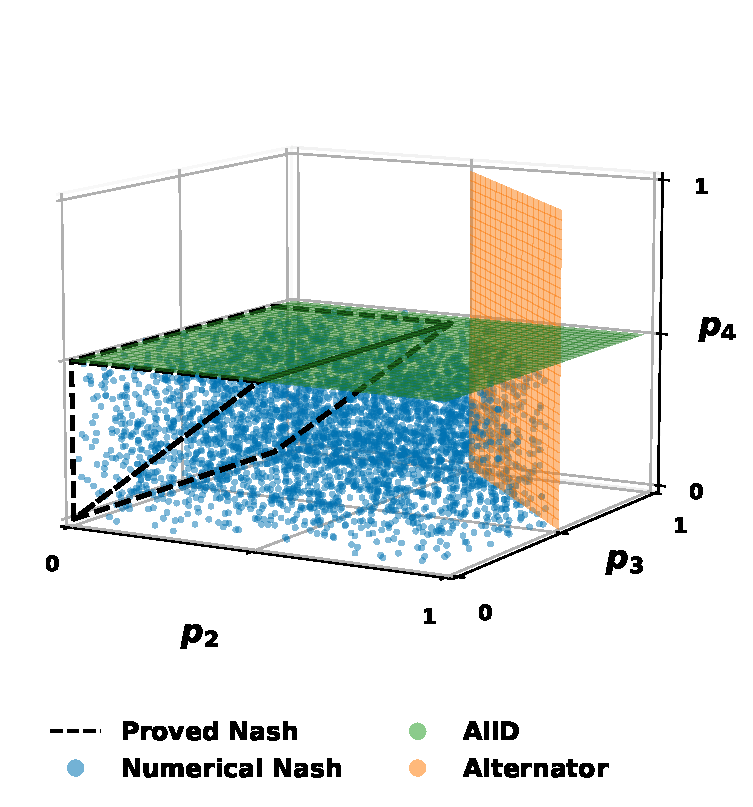
\includegraphics[width=.35\textwidth]{static/for_akin.pdf}
  \caption{\textbf{Nash results for two-bit strategies.} The black dash line
  outlines the space that satisfies conditions (\ref{eq:nash_conditions}). Thus,
  any two-bit reactive strategy that falls within this space is a good strategy.
  We have also numerically explored which agreeable strategies are Nash
  numerically. Namely, for a given agreeable two-bit strategy, and we checked if
  condition \(\pi({\mathbf{q}}, \mathbf{\hat{p}}) \leq (b\!-\!c)\) was satisfied
  against all pure memory-two strategies (\(\mathbf{q} \in \{0, 1\}^{16}\)). We
  recorded if the strategy was Nash or not. We repeated this step for \(10 ^ 4\)
  random strategies. The results indicate that there are strategies that
  are Nash outside the proven space. Note however, that there are two planes
  that constrain the numerical Nash. There are the planes with the equations
  \(\hat{p}_4 = 1 - \frac{c}{b} \text{ and }
  \hat{p}_3 = 1 + \frac{b\!-\!c}{c} - \hat{p}_2\). We obtain these by solving \(\pi(\mathbf{q}, \mathbf{\hat{p}}) =
  (b\!-\!c)\) for \(q \in \{\text{AllD and Alternator}\}\). Parameters: \(c=1, b=2\).
  }\label{fig:two_bit_reactive_nash_results}
\end{figure}

\bibliography{bibliography.bib}

\end{document}